% Problem Formulation (make sure to clearly define S, A, T, and R if you are using an MDP example)'
\section{Problem Formulation}

For this project, we will be working with a labeled gridworld MDP underlying an RL environment. See Fig. \ref{fig: gw_env} for a picture of the proposed gridworld. I am using a labeled gridworld as it will be useful to my work on formal synthesis on the future, and it makes clearer what the task of the robot is, which in this case is \textbf{to get to the goal state (green square) while always avoiding the lava squares (orange, textured).}

\begin{figure}[htbp]
\centerline{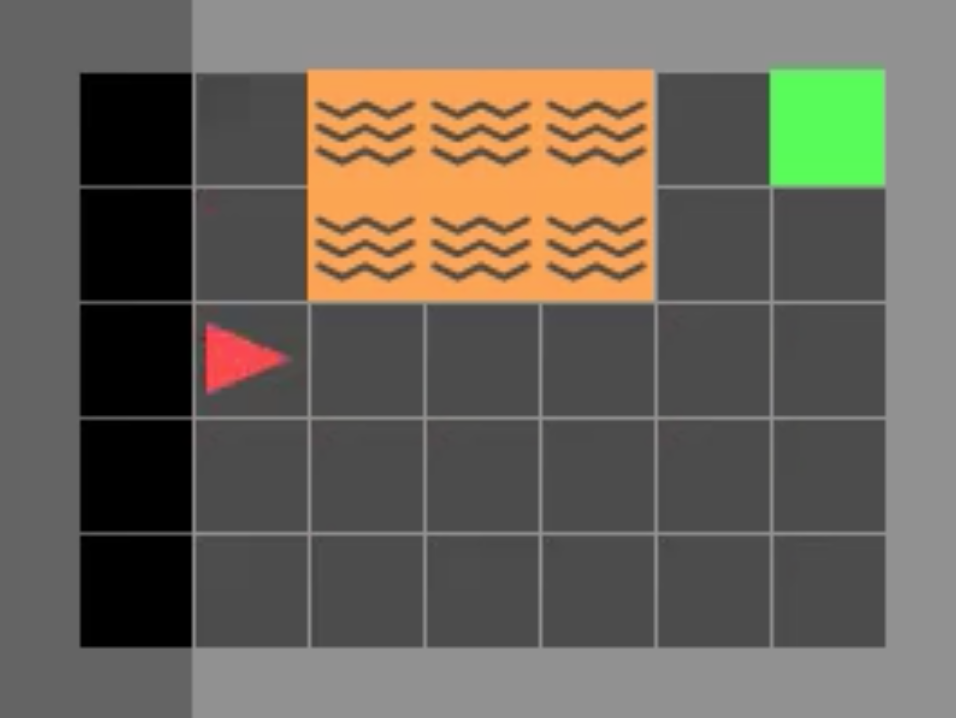
\includegraphics[width=\linewidth]{Figures/gw_env.png}}
\caption{A custom gridworld environment based on the MiniGW Env. \cite{gym_minigrid}}
\label{fig: gw_env}
\end{figure}

The gridworld Labeled MDP is defined as a tuple \(\langle S, A, T, O, L, R, \gamma\rangle:\)\cite{DMU_Book}

\begin{itemize}
    \item \(S\) is the finite set of states. This 9x7 gridworld has a state space consisting of the grid x and y coordinate, along with the agent's direction.
    \item \(A\) is the finite set of actions. Here, the agent can turn $90^{\circ}$ CW, $90^{\circ}$ CCW, or go forward one space in the direction it faces.
    \item \(T: S \times A \rightarrow S\) is the state transition function, where \(T\left(s, a, s^{\prime}\right)\) denotes the probability
\(P\left(s^{\prime} | s, a\right)\) of reaching state \(s^{\prime}\) from state \(s\) by taking action \(a\). Here, the transition uncertainty was simply a 0.05 probability of turning the opposite of the desired direction.
    \item $O$ is the set of possible state observations. For this problem, we let $O = \{\texttt{empty, atGoal, lava}\}$.
    \item $L: S \rightarrow O$ is the labeling function. For our problem, this was used so the agent knew whether the state they were in was in a state labeled \texttt{atGoal} or \texttt{lava}. Again, this will really only be import for formal synthesis.
    \item \(R: S \times A \rightarrow \mathbb{R}\) is the reward function, where \(R(s, a)\) denotes the immediate reward of executing
action \(a\) in state \(s\), whose absolute value is bounded by \(R_{\text {max }}\).  Here, we set the reward function to be 0 everywhere except for at the goal (green square), where the agent will receive a reward $r_{goal} = 1 - 0.9 * (\texttt{number\_of\_steps\_in\_episode} / 100)$. Upon reaching the goal state or the Lava states, the MDP is in a terminal state.
    \item \(\gamma \in[0,1)\) is the discount factor. Here we set $\gamma = 0.99$
\end{itemize}

A policy in MDP is defined as a mapping \(\pi: S \rightarrow A,\) where \(\pi(s)=a\) denotes that action \(a\) is
always executed in state \(s\) following the policy \(\pi .\) The value function of policy \(\pi\) at state \(s\) is the expected discounted return of starting in state \(s\) and executing the policy. The value function can be computed as:
$$
V^{\pi}(s)=R(s, \pi(s))+\gamma \sum_{s^{\prime} \in S} T\left(s, \pi(s), s^{\prime}\right) V^{\pi}\left(s^{\prime}\right)
$$

$$
V^{*}(s)=\max _{a}\left[R(s, a)+\gamma \sum_{s^{\prime} \in S} T\left(s, a, s^{\prime}\right) V^{*}\left(s^{\prime}\right)\right]
$$

It is often useful to express the above equation in terms of \(Q\) -function: \(\pi\) is an optimal policy if and
only if:

$$
\pi(s) \in \underset{a \in A}{\operatorname{argmax}} Q^{\pi}(s, a)
$$

where:
$$
Q^{\pi}(s, a)=R(s, a)+\gamma \sum_{s^{\prime} \in S} T\left(s, a, s^{\prime}\right) V^{\pi}\left(s^{\prime}\right)
$$

Thus, our task was to generate "expert" demonstrations on the grid world environment (MDP defined above) from an expert policy $\pi^*_{expert}$, and then use a GAIL implementation to learn a policy $\pi^*_{GAIL}$ for the Gridworld without access to a reward signal from the environment itself.